% 球谐函数
% 球坐标系|拉普拉斯方程|球谐函数|正交归一性

\pentry{球坐标的拉普拉斯方程\upref{SphLap}, 连带勒让德多项式\upref{AsLgdr}}

当球坐标中的拉普拉斯方程(球坐标系中的拉普拉斯方程\upref{SphLap})分离变量后, 关于极角 $\theta$ 的函数为连带勒让德多项式 $P_l^m(\cos\theta)$, 方向角函数为 $\E^{\I m\phi}$. 我们定义\textbf{球谐函数}为\footnote{有些教材也将球谐函数记为 $Y_l^m$}
\begin{equation}\label{SphHar_eq1}
Y_{l, m} (\uvec r) = Y_{l, m}(\theta, \phi) = A_{l,m} P_l^m(\cos \theta) \E^{\I m\phi}
\end{equation}
其中 $l, m$ 为整数, $l \ge 0$, $-l \le m \le -l$. $A_{l,m}$ 是归一化系数, 使得 $\abs{Y_{l, m} (\uvec r)}^2$ 在单位球面上的面积分等于 1\footnote{\autoref{SphHar_eq2} 是 Mathematica 中的定义, 也有一种定义在前面加 $(-1)^m$, 同样满足归一化条件.}.
\begin{equation}\label{SphHar_eq2}
A_{l,m} =  \sqrt{\frac{2l + 1}{4\pi }\frac{(l - m)!}{(l + m)!}}
\end{equation}
球谐函数可以看作是将单位球面上的每一点(或者三维空间中的每个方向)映射到一个复数函数值.

\begin{figure}[ht]
\centering
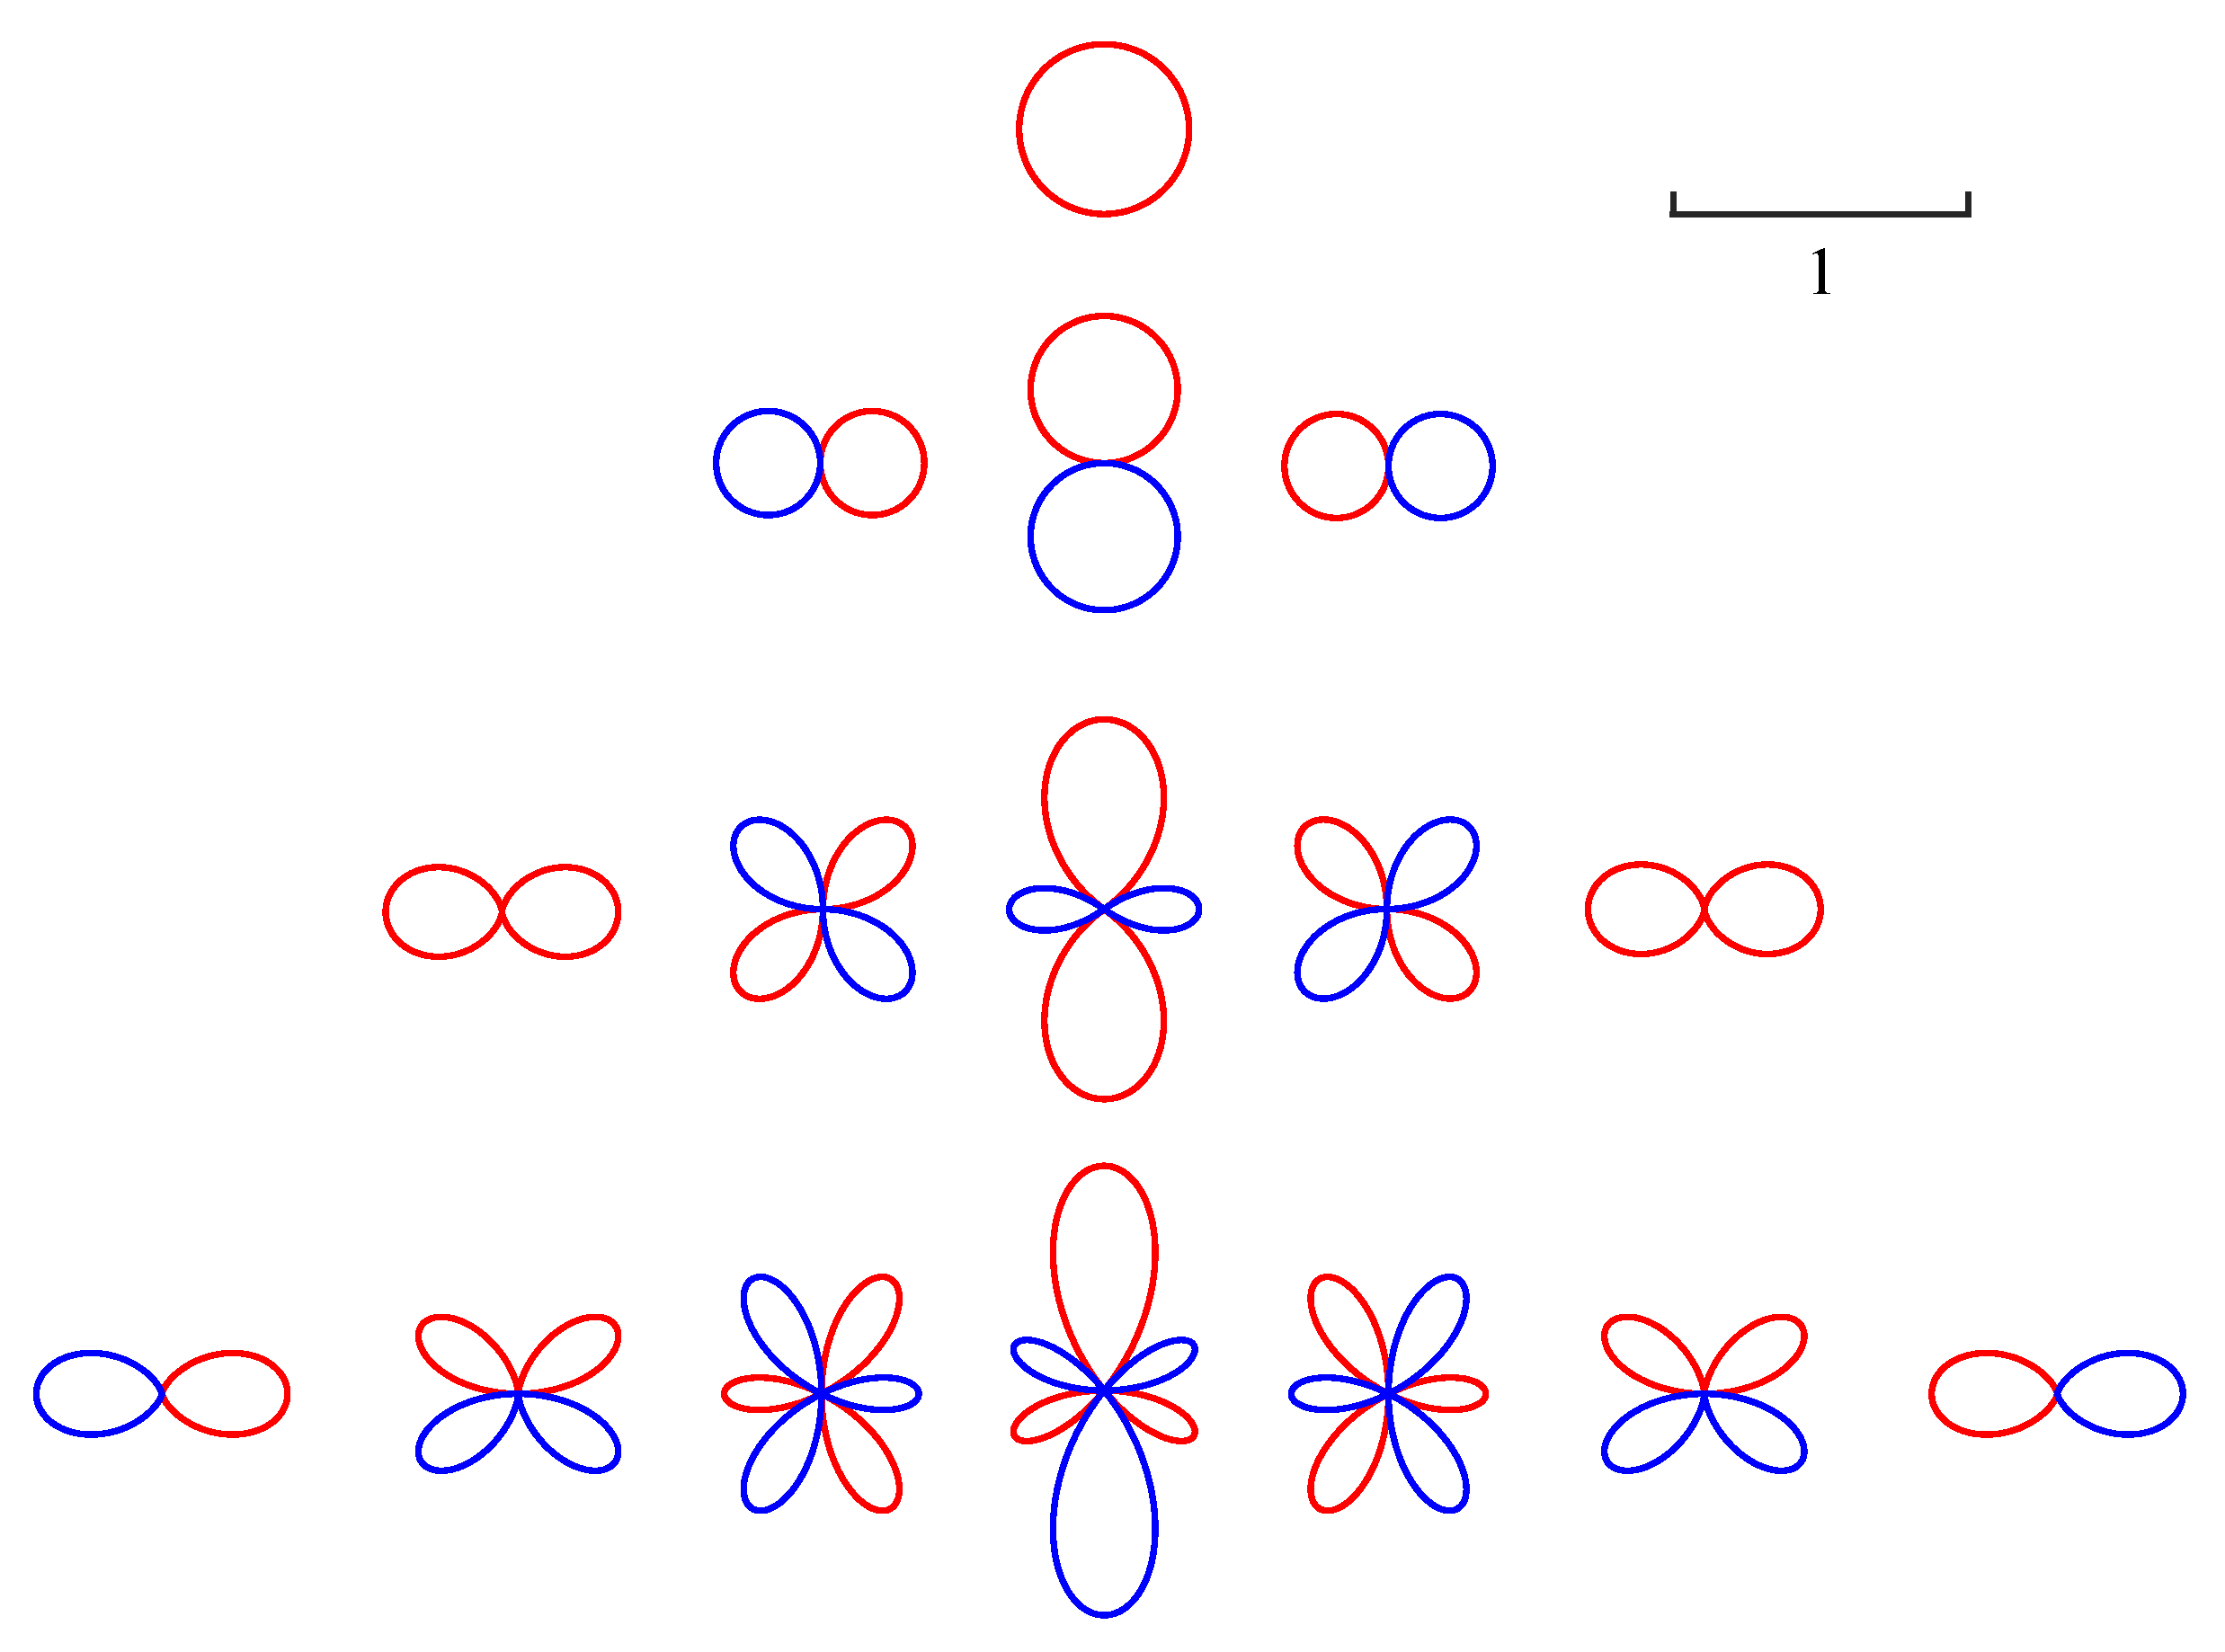
\includegraphics[width=10cm]{./figures/SphHar_1.pdf}
\caption{$r(\theta) = \abs{Y_{l,m}(\theta, 0)}$ 的极坐标曲线, 注意 $Y_{l,m}(\theta, 0)$ 是实数. 红色代表 $Y_{l,m}(\theta, 0) > 0$, 蓝色代表 $Y_{l,m}(\theta, 0) < 0$. 第 1 行到第 4 行分别为 $l = 0$ 到 $3$, 每行从左到右分别为 $m = -l$ 到 $l$. 图中的右上角标明了 $r$ 的单位长度. 这里的球谐函数使用了 Condon–Shortley 相位(见下文).} \label{SphHar_fig1}
\end{figure}

\subsection{偏微分方程}
球谐函数是偏微分方程
\begin{equation}
\qty[\frac{1}{\sin\theta}\pdv{\theta} \qty(\sin \theta \pdv{\theta}) + \frac{1}{\sin^2 \theta} \qty(\pdv[2]{\phi})]Y_{lm}(\theta, \phi) = -l(l+1)Y_{lm}(\theta, \phi)
\end{equation}
的解. 中括号中的算符是球坐标系拉普拉斯算子 $\laplacian$ 中的角向部分(记为 $\laplacian_\Omega$)乘以 $r^2$. 常见的球谐函数见 “球谐函数列表\upref{YlmTab}”.

\subsection{归一化系数}
由球谐函数的归一化条件, % 未完成:哪里讲解一下立体角是单位球面上的面积元, 以及极坐标中的表达式. % 链接未完成
\begin{equation}\ali{
1 &= \int \abs{Y_{l, m}(\uvec r)}^2 \dd{\Omega} = \int_0^\pi  \int_0^{2\pi}  \abs{Y_{l, m}(\theta, \phi)}^2 \sin\theta\dd{\theta}\dd{\phi} \\
&= \abs{A_{l,m}}^2 \int_{-1}^1  \abs{P_l^m(\cos\theta)}^2 \dd{(\cos \theta)} \int_0^{2\pi } \abs{\E^{\I m\phi}}^2  \dd{\phi}\\
&= \frac{2\pi}{\abs{A_{l,m}'}^2} \abs{A_{l,m}}^2
}\end{equation}
其中 $A_{l,m}'$ 是 $P_l^m(x)$ 的归一化系数(见\autoref{AsLgdr_eq3}~\upref{AsLgdr}), 代入后可得 $A_{l,m}$.

\subsection{Condon–Shortley 相位}
与连带勒让德多项式相同, 在定义球谐函数时我们也可以选择是否包含 \textbf{Condon–Shortley 相位} $(-1)^m$(物理中一般选择包含). 如果包含, 我们可以选择将其包含在连带勒让德多项式中(如\autoref{AsLgdr_eq1}~\upref{AsLgdr}), 或者包含在球谐函数的定义中. 如果不包含, 该相位在两个定义中都不出现.

\subsection{正交归一性}
由勒让德函数的正交归一性(\autoref{AsLgdr_eq4}~\upref{AsLgdr})以及 $\E^{\I m \phi}$  的正交归一性,% 未完成: 引用复数傅里叶级数中的公式
 不难证明球谐函数的正交归一性
\begin{equation}
\int Y_{l', m'}(\uvec r) Y_{l, m} (\uvec r) \dd{\Omega} = \delta_{ll'}\delta_{mm'}
\end{equation}

\subsection{其他性质}
\begin{equation}\label{SphHar_eq6}
Y_{l,-m}(\uvec r) = (-1)^m Y_{l,m}(\uvec r)^*
\end{equation}
这里的 $(-1)^m$ 是由连带勒让德多项式的性质而来, 而共轭由 $\exp(\I m\phi)$ 因子而来.

\subsubsection{旋转变换}
\begin{equation}
Y_{l,m}(\uvec r') = \sum_{m'=-l}^l D_{m,m'}^{(l)} (\mathcal R)^* Y_{l,m'}(\uvec r)
\end{equation}
其中 $\mat D^{(l)}$ 是 Wigner D 矩阵\upref{WigDmt}. 从量子力学的角度来说, 总角动量是与方向无关的, 只有角动量在某方向的分量有关.

\subsection{中心对称}
$l$ 为偶数时, 球谐函数是中心对称的(偶宇称\upref{IntPry}), 否则是反对称的(奇宇称).
\begin{equation}\label{SphHar_eq8}
Y_{l,m}(-\uvec r) = (-1)^l Y_{l,m}(\uvec r)
\end{equation}
可以用\autoref{SphHar_fig1} 验证.

\subsection{积分}
三个球谐函数之积的积分可以表示成两个 CG 系数\upref{SphCup}或 3j 符号\upref{ThreeJ}相乘\footnote{见 Bransden 附录 A4, 以及 Wikipedia 的 3j/CG coefficients 页面}
\begin{equation}\label{SphHar_eq3}
\ali{
&\quad \int Y_{l_1 m_1} (\uvec r) Y_{l_2 m_2} (\uvec r) Y_{l_3 m_3}(\uvec r) \dd{\Omega}\\
&= (-1)^{m_3} \sqrt{\frac{(2l_1+1)(2l_2+1)}{4\pi(2l_3+1)}} \bmat{l_1& l_2& l_3\\ 0 & 0 & 0}\bmat{l_1 & l_2 & l_3\\  m_1 & m_2 & -m_3}\\
&= \sqrt{\frac{(2l_1+1)(2l_2+1)(2l_3+1)}{4\pi}}  \pmat{l_1& l_2& l_3\\ 0 & 0 & 0}\pmat{l_1 & l_2 & l_3\\  m_1 & m_2 & m_3}
}\end{equation}

\subsection{应用}
见平面波的球谐展开\upref{Pl2Ylm} 和电多极子展开\upref{EMulPo}.
